%%*****************************************************************************%%
%																				%
%																				%
%								LEAVE ME HERE									%
%																				%
%																				%
%              _____ ______   ________                   _______   				%  
%             |\   _ \  _   \|\   __  \                 /  ___  \    			%
%             \ \  \\\__\ \  \ \  \|\  \  ____________ /__/|_/  /|   			%
%              \ \  \\|__| \  \ \   _  _\|\____________\__|//  / /   			%
%               \ \  \    \ \  \ \  \\  \\|____________|   /  /_/__  			%
%                \ \__\    \ \__\ \__\\ _\                |\________\			%
%                 \|__|     \|__|\|__|\|__|                \|_______|			%
%                                                      							%
%																				%
%%*****************************************************************************%%
%									Links										%
%																				%
%		x Read only : https://www.overleaf.com/read/pqwrvyrykrsh				%
%		x Edit&Read : https://www.overleaf.com/6786843srbkbx					%
%		x Github	: https://www.github.com/MR-2								%
%																				%
%%*****************************************************************************%%
%							About - This Document								%
%																				%
%		x	 Digital Amplitude Modulation Plot Sample							%
%																				%
%		Note: Use it however you want.											%
%																				%
%%*****************************************************************************%%
%									Setup										%
%																				%
\documentclass[tikz,border=10pt]{standalone}
\begin{document}
    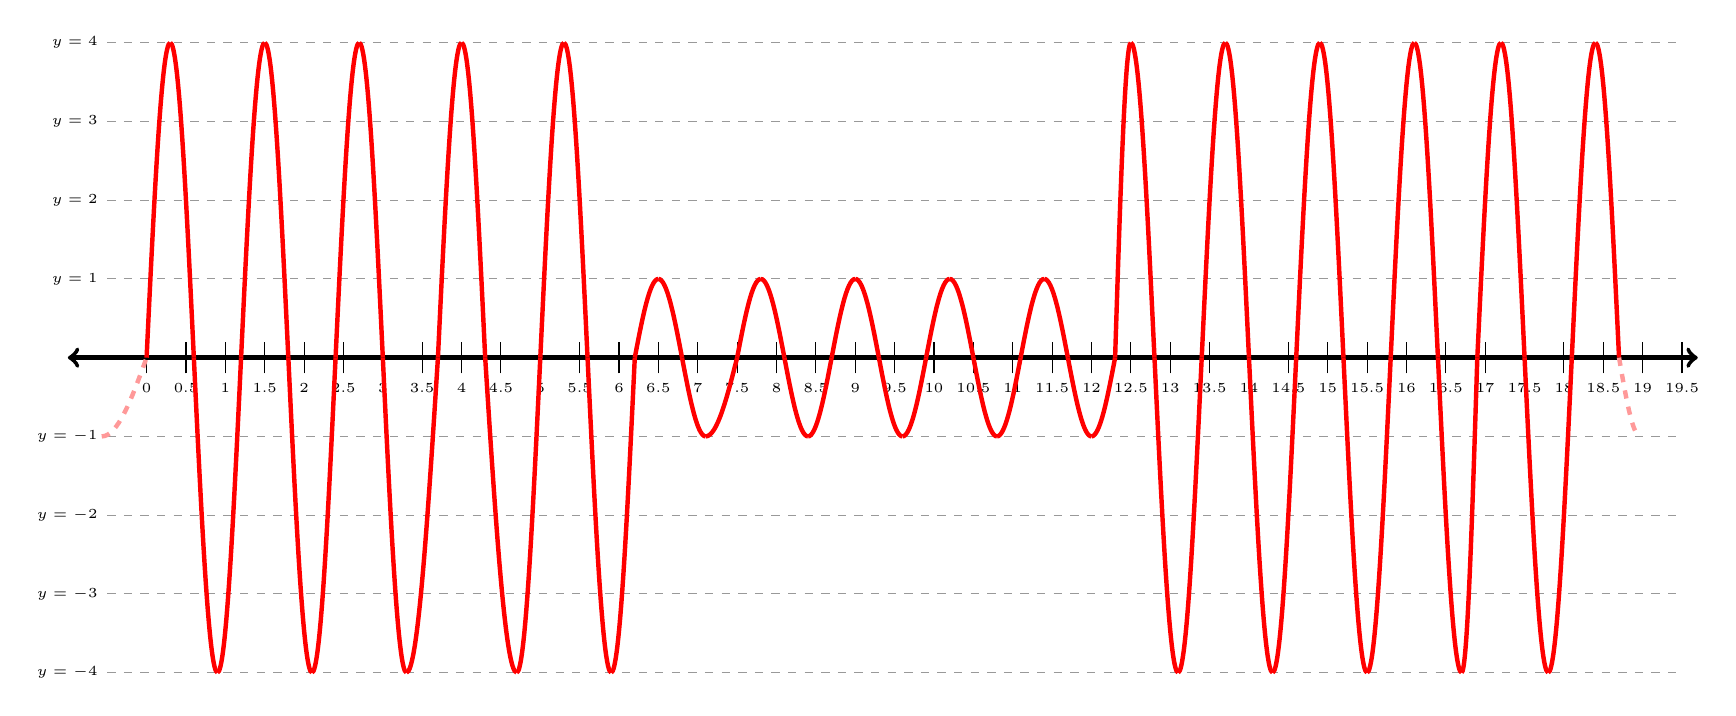
\begin{tikzpicture}
    \draw[ultra thick, black,<->] (-1,0) -- (19.7,0);
    \draw[dashed,draw=black!40] (-0.5,1)node[left,font=\tiny] {$y=1$} -- (19.5,1);
    \draw[dashed,draw=black!40] (-0.5,-1)node[left,font=\tiny] {$y=-1$} -- (19.5,-1); 
    \draw[dashed,draw=black!40] (-0.5,2)node[left,font=\tiny] {$y=2$} -- (19.5,2);
    \draw[dashed,draw=black!40] (-0.5,-2)node[left,font=\tiny] {$y=-2$} -- (19.5,-2); 
    \draw[dashed,draw=black!40] (-0.5,3)node[left,font=\tiny] {$y=3$} -- (19.5,3);
    \draw[dashed,draw=black!40] (-0.5,-3)node[left,font=\tiny] {$y=-3$} -- (19.5,-3);
    \draw[dashed,draw=black!40] (-0.5,4)node[left,font=\tiny] {$y=4$} -- (19.5,4);
    \draw[dashed,draw=black!40] (-0.5,-4)node[left,font=\tiny] {$y=-4$} -- (19.5,-4);
    \foreach \x in {0,0.5,...,19.5}{
    \draw (\x,-0.2)node [below,font=\tiny,] {\x} -- (\x,0.2) ;
    }
    
    
    \draw[ultra thick,dashed, red!40] (-0.57,-1) cos (0,0);
    
    \draw[ultra thick, red] (0,0) sin (0.3,4);
    \draw[ultra thick, red] (0.3,4) cos (0.6,0);
    \draw[ultra thick, red] (0.6,0) sin (0.9,-4);
    \draw[ultra thick, red] (0.9,-4) cos (1.2,0);
    
	\draw[ultra thick, red] (1.2,0) sin (1.5,4);
    \draw[ultra thick, red] (1.5,4) cos (1.8,0);
    \draw[ultra thick, red] (1.8,0) sin (2.1,-4);
    \draw[ultra thick, red] (2.1,-4) cos (2.4,0);
    
    \draw[ultra thick, red] (2.4,0) sin (2.7,4);
    \draw[ultra thick, red] (2.7,4) cos (3,0);
    \draw[ultra thick, red] (3,0) sin (3.3,-4);
    \draw[ultra thick, red] (3.3,-4) cos (3.7,0);
    
    \draw[ultra thick, red] (3.7,0) sin (4,4);
    \draw[ultra thick, red] (4,4) cos (4.3,0);
    \draw[ultra thick, red] (4.3,0) sin (4.7,-4);
    \draw[ultra thick, red] (4.7,-4) cos (5,0);
    
    \draw[ultra thick, red] (5,0) sin (5.3,4);
    \draw[ultra thick, red] (5.3,4) cos (5.6,0);
    \draw[ultra thick, red] (5.6,0) sin (5.9,-4);
    \draw[ultra thick, red] (5.9,-4) cos (6.2,0);
    
    %%%%Onesisssss
    \draw[ultra thick, red] (6.2,0) sin (6.5,1);
    \draw[ultra thick, red] (6.5,1) cos (6.8,0);
    \draw[ultra thick, red] (6.8,0) sin (7.1,-1);
    \draw[ultra thick, red] (7.1,-1) cos (7.5,0);
    
    \draw[ultra thick, red] (7.5,0) sin (7.8,1);
    \draw[ultra thick, red] (7.8,1) cos (8.1,0);
    \draw[ultra thick, red] (8.1,0) sin (8.4,-1);
    \draw[ultra thick, red] (8.4,-1) cos (8.7,0);
    
    \draw[ultra thick, red] (8.7,0) sin (9,1);
    \draw[ultra thick, red] (9,1) cos (9.3,0);
    \draw[ultra thick, red] (9.3,0) sin (9.6,-1);
    \draw[ultra thick, red] (9.6,-1) cos (9.9,0);
    
    \draw[ultra thick, red] (9.9,0) sin (10.2,1);
    \draw[ultra thick, red] (10.2,1) cos (10.5,0);
    \draw[ultra thick, red] (10.5,0) sin (10.8,-1);
    \draw[ultra thick, red] (10.8,-1) cos (11.1,0);
    
    \draw[ultra thick, red] (11.1,0) sin (11.4,1);
    \draw[ultra thick, red] (11.4,1) cos (11.7,0);
    \draw[ultra thick, red] (11.7,0) sin (12,-1);
    \draw[ultra thick, red] (12,-1) cos (12.3,0);
    
    %% fourssies
    \draw[ultra thick, red] (12.3,0) sin (12.5,4);
    \draw[ultra thick, red] (12.5,4) cos (12.8,0);
    \draw[ultra thick, red] (12.8,0) sin (13.1,-4);
    \draw[ultra thick, red] (13.1,-4) cos (13.4,0);
    
	\draw[ultra thick, red] (13.4,0) sin (13.7,4);
    \draw[ultra thick, red] (13.7,4) cos (14,0);
    \draw[ultra thick, red] (14,0) sin (14.3,-4);
    \draw[ultra thick, red] (14.3,-4) cos (14.6,0);
    
    \draw[ultra thick, red] (14.6,0) sin (14.9,4);
    \draw[ultra thick, red] (14.9,4) cos (15.2,0);
    \draw[ultra thick, red] (15.2,0) sin (15.5,-4);
    \draw[ultra thick, red] (15.5,-4) cos (15.8,0);
    
    \draw[ultra thick, red] (15.8,0) sin (16.1,4);
    \draw[ultra thick, red] (16.1,4) cos (16.4,0);
    \draw[ultra thick, red] (16.4,0) sin (16.7,-4);
    \draw[ultra thick, red] (16.7,-4) cos (16.9,0);
    
    \draw[ultra thick, red] (16.9,0) sin (17.2,4);
    \draw[ultra thick, red] (17.2,4) cos (17.5,0);
    \draw[ultra thick, red] (17.5,0) sin (17.8,-4);
    \draw[ultra thick, red] (17.8,-4) cos (18.1,0);
    \draw[ultra thick, red] (18.1,0) sin (18.4,4);
    \draw[ultra thick, red] (18.4,4) cos (18.7,0);
    
    
    
    \draw[ultra thick,dashed, red!40] (18.7,0) sin (18.97,-1);
    
    \end{tikzpicture}
\end{document}